%
% Draft  document depthandcurv.tex
% Looks at depth, straight length, and curved length of follicles
%
 
\documentclass[titlepage]{article}  % Latex2e
\usepackage{graphicx,lscape,subfigure}
\usepackage{tikz}
\usepackage{bm,longtable}
\usepackage{textcomp}
 

\title{Follicle depth, straight length, and curved length in plain and wrinkly sheep}
\author{Jim Watts and Neville Jackson}
\date{27 Aug 2018} 

 
\begin{document} 


 
\maketitle      
\tableofcontents

$\newcommand{\E}{\mathrm{E}}$
$\newcommand{\Var}{\mathrm{Var}}$
$\newcommand{\Cov}{\mathrm{Cov}}$ 
$\newcommand{\SD}{\mathrm{SD}}$ 

\clearpage
\section{Introduction} 

\section{Materials and Methods}
\subsection{Sheep studied}
This is a small study of 36 sheep from two Flocks, 18 from each Flock. Wthin each Flock there were 9 sheep chosen to represent the "loose" Skintype, and 9 sheep chosen to represent the "wrinkly" Skintype. 

On each sheep 25 follicles chosen at random were measured on a vertical skin section taken fron a skin biopsy sample obtained by the technique of Maddocks and Jackson (1988)~\cite{madd:88}. The measurements were of follicle depth, $t$, and $h$, as defined below.

\subsection{Measurements}
The following measurements and scores were available
\begin{description}
\item[SkinType] visual scores for sheep skin type. Two grades "loose" and "wrinkly". 
\item[Follicle depth] perpendicular distance from skin surface to bottom of follicle bulb
\item[Follicle straight length(t)] distance from skin surface to bottom of follicle bulb, measured at the angle of the follicle to the surface.
\item[Follicle sagitta(h)] If the straight follicle length is considered to be the chord of a circle, the sagitta is the height of the arc above the centre of the chord.
\end{description}

From these measurements it was possible to calculate
\begin{description}
\item[Radius of curvature of follicle]  given by $R = h/2 + t^{2}/(8h)$
\item[Angle subtended by the arc] given by $\theta = 2 asin(2/(2R))$
\item[Follicle curved length] given by $S = R \theta$
\end{description}

The measurement of fibre curvature used by the wool industry is the reciprocal of radius of curvature and is in degrees per mm. The reciprocal of our $R$ would be in radians per mm.

\subsection{Statistical analysis}

Data were imported into the R statistical program~\cite{rprog:13} and analysed using the {\em aov()} function for analysis of variance.

\section{Results}
\subsection{Means}
Means for each Skintype within each Flock are given in Table~\ref{tab:means}
%\documentclass{article}
%\usepackage{lscape}
%\usepackage{tablefootnote}
%\begin{document}

\begin{table}[ht]
\centering
\caption{Means for follicle measurements separately for each Flock and each Skintype}
\label{tab:means}
\vspace{0.1in}
\begin{tabular}{|p{0.5in}|p{0.6in}|p{0.6in}|p{0.6in}|p{0.6in}|p{0.6in}|} \hline
  Flock & Skin.type & Folldepth & Straightlen & Curvlen  & Radcurv\\   
    \hline
  1 & loose & 1.579 & 1.827 & 1.839 & 6.97  \\ 
  2 & loose & 1.721 & 1.846 & 1.854 & 8.99  \\ 
  1 & wrinkly & 1.972 & 2.136 & 2.222 & 2.92 \\ 
  2 & wrinkly & 1.833 & 1.925 & 2.035 & 2.15  \\ 
   \hline
\end{tabular}
\end{table}

%\end{document}



All four traits ( Follicle depth, straight follicle lenfgth, curved follicle length, and radius of curvature) would appear to differ substantially between loose and wrinkly Skintypes, but the two Flocks would seem to be similar.

We do not present standard deviations or standard errors here.  The experimental design has multiple error levels. There are two random effects, Sheep, and Follicles within Sheep. Each of these contributes to the standard error of a mean. We need to estimate variance components for Sheep and Follicles to do the standard errors properly. 

However we can test the significance of the Skintype difference and the Flock difference with an appropriate analysis of variance. We show these analyses of variance in Table~\ref{tab:aov}
%FOLLDEP
\label{tab:aov}
\begin{table}[ht]
\centering
\caption{Analyses of variance of Follicle depth, Follicle straight length, Follicle curved length, and Follicle radius of curvature}
\begin{tabular}{lrrrrr}
  \hline
 & & Follicle depth & & & \\
 Effect & Df & Sum Sq & Mean Sq & F value & Pr($>$F) \\ 
  \hline
  Error: Sheep & & & & &  \\
Flock     & 1 & 1.08 & 1.08 & 0.00 & 0.9861 \\ 
  Skin.type & 1 & 35822.56 & 35822.56 & 10.16 & 0.0031 \\ 
  Residuals & 33 & 116320.51 & 3524.86 &  &  \\ 
  Error: Within & & & & &  \\
  Residuals1 & 860 & 59641.23 & 69.35 &  &  \\ 
   \hline
%\end{tabular}
%\end{table}

%STRAIGHTLEN
%\begin{table}[ht]
%\centering
%\begin{tabular}{lrrrrr}
% \hline
 & & Follicle straight length & & & \\
 Effect & Df & Sum Sq & Mean Sq & F value & Pr($>$F) \\ 
  \hline
  Error: Sheep & & & & &  \\
Flock     & 1 & 5218.12 & 5218.12 & 1.32 & 0.2591 \\ 
  Skin.type & 1 & 21042.58 & 21042.58 & 5.32 & 0.0275 \\ 
  Residuals & 33 & 130612.06 & 3957.94 &  &  \\ 
  Error: Within & & & & &  \\
  Residuals1 & 860 & 66226.12 & 77.01 &  &  \\ 
   \hline
%\end{tabular}
%\end{table}

%CURVLEN
%\begin{table}[ht]
%\centering
%\begin{tabular}{lrrrrr}
% \hline
 & & Follicle curved length & & & \\
 Effect & Df & Sum Sq & Mean Sq & F value & Pr($>$F) \\ 
  \hline
  Error: Sheep & & & & &  \\
Flock     & 1 & 4251.50 & 4251.50 & 1.03 & 0.3180 \\ 
  Skin.type & 1 & 44711.74 & 44711.74 & 10.81 & 0.0024 \\ 
  Residuals & 33 & 136454.62 & 4134.99 &  &  \\ 
  Error: Within & & & & &  \\
  Residuals1 & 860 & 75424.61 & 87.70 &  &  \\ 
   \hline
%\end{tabular}
%\end{table}

%RADCURV
%\begin{table}[ht]
%\centering
%\begin{tabular}{lrrrrr}
% \hline
 & & Follicle radius of curvature & & & \\
 Effect & Df & Sum Sq & Mean Sq & F value & Pr($>$F) \\ 
  \hline
  Error: Sheep & & & &  & \\
Flock     & 1 & 239208.35 & 239208.35 & 1.31 & 0.2603 \\ 
  Skin.type & 1 & 16554724.49 & 16554724.49 & 90.79 & 0.0000 \\ 
  Residuals & 33 & 6017368.02 & 182344.49 &  &  \\ 
  Error: Within & & & & &  \\
  Residuals1 & 860 & 20509483.53 & 23848.24 &  &  \\ 
   \hline
\end{tabular}
\end{table}

The first thing to note is that there are multiple error levels - corresponding to variation between sheep and variation between follicles within a sheep. The appropriate error level for testing Flock and Skintype differences is Error:Sheep - the line labelled Residuals. We can see that the analyses have used this error level for the F tests. These show that the Skintype difference was significant for all four traits, althought the probability level for Follicle straight length was only .027 ( ie between 1 percent and five percent significance). None of the four traits showed a significant Flock difference. 

This result is , of course, what we expected to find.  Based on our understanding of the histology of wrinkle formation, we expect that wrinkled sheep will have a layer of hard collagen in the dermis which interferes with the downward growth of follicles from the dermis ( ie reduces their length) and which also causes the downgrowing follicles to curve sideways in an attempt to complete their length growth ( ie increases Radius of curvature).  So these results support our hypothesis regarding the role of collagen in wrinkle formation and its effect on developing follicles.

\subsection{Variance components}
With two Error levels ( Sheep and Follicles within sheep) we need to estimate variance components for each level, in order to calculate the standard error of a mean.  In Table~\ref{tab:aov} the mean square for Residual1 is the Follicles withn sheep variance component$(\sigma^{2}_{F})$. To get the Sheep variance component $\sigma^{2}_{S}$ we calculate
\begin{displaymath}
\sigma^{2}_{S} = (MS(sheep) - MS(follicles within sheep)) / N_{F}
\end{displaymath}
where $N_{F}$ is the number of follicles per sheep.

We can then calculate the variance of a mean as
\begin{displaymath}
Var(mean) = \sigma^{2}_{S}/N_{S} + \sigma^{2}_{F}/(N_{S} N_{F})
\end{displaymath}
where $N_{S}$ is number of sheep in the mean and $N_{F}$ is number of follicles per sheep.
This gives the variance of a mean. To get a standard error we take its square root.

Table~\ref{tab:se} gives the variance component estimates calculated as above  for each of the four traits, plus a standard error calculated for a mean of 9 sheep with 25 follicles per sheep.
%\documentclass{article}
%\usepackage{lscape}
%\usepackage{tablefootnote}
%\begin{document}

\begin{table}[ht]
\centering
\caption{Sheep and follicle within sheep variance components for four traits. Standard error of a mean of 9 sheep with 25 follicles per sheep}
\label{tab:se}
\vspace{0.1in}
\begin{tabular}{|p{1.6in}|p{0.6in}|p{0.6in}|p{0.6in}|p{0.6in}|} \hline
   & Folldepth & Straightlen & Curvlen  & Radcurv\\   
    \hline
 Sheep component & 138.22 & 155.24 & 161.89 & 6339 \\
 Follicles component & 69.35 & 77.01 & 87.70 & 23848\\
 Standard error of mean & 3.95 & 4.19 & 4.28 & 28.46\\
   \hline
\end{tabular}
\end{table}

%\end{document}



These are the standard errors which apply to the means given in Table~\ref{tab:means} The significance tests in Table~\ref{tab:aov} indicate a higher level of significance because they are for the Skintype difference averaged across both Flocks - ie they correspond to means of 18 Sheep rather than 9. We have not presented the means for Skintype differences averaged across both Flocks, so we present these and their standard errors in Table~\ref{tab:skintype}
%\documentclass{article}
%\usepackage{lscape}
%\usepackage{tablefootnote}
%\begin{document}

\begin{table}[ht]
\centering
\caption{Means and standard errors for follicle measurements separately for each  Skintype}
\label{tab:skintype}
\vspace{0.1in}
\begin{tabular}{|p{0.6in}|p{0.6in}|p{0.6in}|p{0.6in}|p{0.6in}|} \hline
   Skin.type & Folldepth & Straightlen & Curvlen  & Radcurv\\   
    \hline
  Mean loose & 82.5 & 91.86 & 92.32 & 399.0  \\ 
  Mean wrinkly & 95.14 & 101.6 & 106.5 & 127.1 \\ 
  Standard error & 2.79 & 2.96 & 3.03 & 20.12  \\ 
   \hline
\end{tabular}
\end{table}

%\end{document}



We see that these means are indeed significantly different, as indicated in the analyses of variance in Table~\ref{tab:aov}.

\subsection{Correlations}
Figure~\ref{fig:curvlenxfd} shows a scatterplot of curved length of follicles against follicle depth.
%\documentclass{article}
%\usepackage{graphicx,subfigure}
%\begin{document}

\begin{figure}[!h]
  \centering
  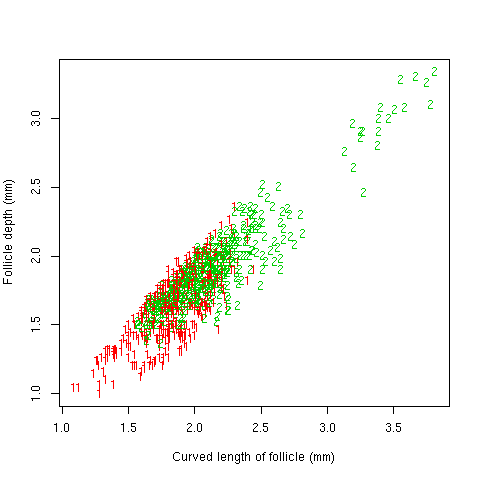
\includegraphics[width=1.0\textwidth]{curvlenxfd.png}
  \caption{Plot of follicle depth against curved length of follicles. The loose and wrinkly skintypes are shown as points labelled 1 ( red) and 2(green) respectively.}
  \label{fig:curvlenxfd}
\end{figure}

%\end{document}


 It suggests that follicle depth is a rather poor indicator of the curved length of a follicle. The points seem to cluster at or below the 1 to 1 line, indicating that curved length is either equal to or longer than follicle depth, depending on how much the follicle is curved. In this situation a correlation is not a good descriptor. 

Figure~\ref{fig:curvlenxt} shows a similar scatterplot of curved length against straight length of follicles.
%\documentclass{article}
%\usepackage{graphicx,subfigure}
%\begin{document}

\begin{figure}[!h]
  \centering
  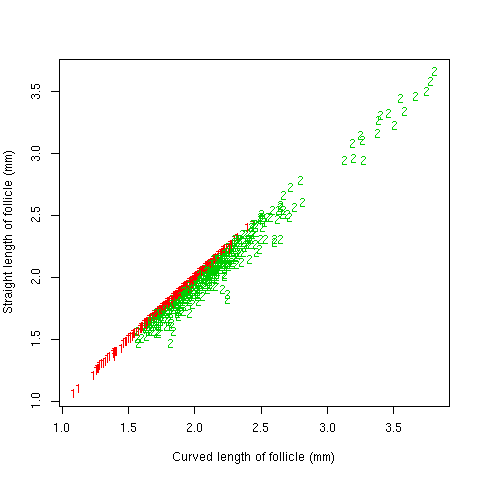
\includegraphics[width=1.0\textwidth]{curvlenxt.png}
  \caption{Plot of  straight length against curved length of follicles. The loose and wrinkly skintypes are shown as points labelled 1 ( red) and 2(green) respectively.}
  \label{fig:curvlenxt}
\end{figure}

%\end{document}


 We see a similar picture to Figure~\ref{fig:curvlenxfd} but with much closer agreement. The points again cluster at or below the 1 to 1 line. Curved length is either equal to straight length or slightly longer. Straight length is a better indicator of curved length than is follicle depth, but it misses out if the follicles are curved.

Figure~\ref{fig:radcurvxcurvlen} shows a scatterplot of curved length against radius of curvature.
%\documentclass{article}
%\usepackage{graphicx,subfigure}
%\begin{document}

\begin{figure}[!h]
  \centering
  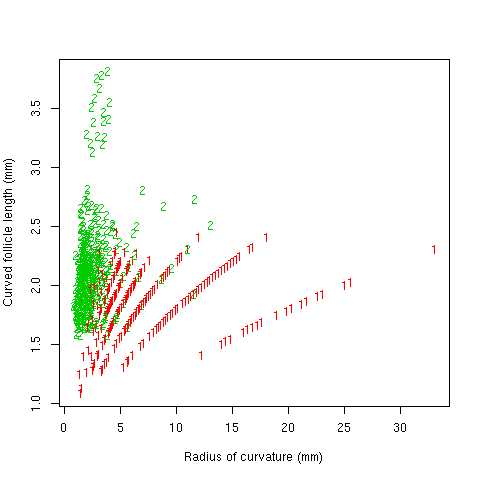
\includegraphics[width=1.0\textwidth]{radcurvxcurvlen.png}
  \caption{Plot of  radius of curvature against curved length of follicles. The loose and wrinkly skintypes are shown as points labelled 1 ( red) and 2(green) respectively.}
  \label{fig:radcurvxcurvlen}
\end{figure}

%\end{document}


Here we see something radically diffferent. Why the stepped spacing of points, especially those from the loose Skintype with high radius of curvature. Well, the issue is that measuring the follicle sagitta (h) gets to be rather imprecise when the follicle is not curved. Values of 1, 2, 3 for the sagitta produce the grouping effect when converted to radius of curvature.

What Figure~\ref{fig:radcurvxcurvlen} shows is that wrinkly sheep have curved follicles that may also be long, while loose sheep have straighter follicles that on average are shorter.
This is not quite what we expected. Those very long follicles in the wrinkly group bear further investigation.

The relationship between length and curvature is complicated. The points occupy the bottom left corner of the plot. Clearly there are other factors involved. 

\clearpage
\section{Discussion}
We wanted to show that wrinkled sheep have curved follicles, and we wanted to use something other than a subjective score for follicle curvature. We have achieved that - the radius of curvature differs significantly between loose and wrinkly sheep.

There are also differences in follicle length, regardless of how it is measured. The wrinkled sheep have longer follicles. This begs an explanation. If the presence of collagen in wrinkled sheep interferes with follicle development causing them to grow curved, that is one thing. But how would presence of collagen cause follicles to grow longer? Perhaps the folding of the epidermal and dermal layers which occurs as wrinkles form 'stretches' the follicles. Perhaps the collagen contracts and pulls on the follicles. Perhaps it is not a simple physical effect at all. Perhaps the collagen moves the papilla cells toward which the follicle downgrowth develops, so that the intital infolding of the epidermis and the papilla cells get out of line, causing the follicle to both curve sideways and grow longer in order to reach the papilla cells. We do not know.

So what needs to be done from here? Well we need to sort out whether the length of follicles is at all important in relation to fibre growth. There has been one experiment selecting for follicle depth (Jackson (2017)~\cite{jack:17a}) and it was a failure in relation to improving wool production.  It changed follicle depth and fibre diameter and variance of fibre diameter. The experiment was started when there was a feeling that 'deep' follicles had a better blood supply and a more vigorous wool growth. That sort of thinking has since disappeared. 'Deep' follicles are just long follicles, not anything special. Having an elongted shaft is not going to help a follicle grow more wool.

There also needs to be some consideration as to whether follicle curvature is the same thing as intrinsic fibre curvature, and whether the current commercial curvature measurement technology ( Laserscan or OFDA) measures intrinsic fibre curvature. It comes down to whether follicle curvature is the only factor determining intrinsic fibre curvature, or whether there are other  factors perhaps related to the fibre cross sectional distribution of cortical cell types. Understanding the effect of collagen on follicle curvature is a half-way house. We need to know the effect of collagen on intrinsic fibre curvature, not the 'set' we observe in staple crimp, not some 'set' we measure under Laserscan od OFDA standardised measuring conditions, but the real intrincic curvature which is wahat a fibre can always be relaxed to and which is determined by different growth rates of the ortho and para cortical cells in a fibre with a bilaterally segmented cortex.

That being said, this study has progressed our understanding of why sheep with wrinkle and hard collagen differ from plain bodied sheep in wool growth. They differ because the presence of a layer of hard collagen in the dermis affects the size and shape of wool follicles. In our discussion we have explored possible mechanisms.

\section{Conclusion}
Of all the aspects discussed above, one stands out. Here is what we think is actually happening to follicle development in wrinkly sheep.

Follicles develop in the foetus between 60 and 150 days. Papilla cells migrate to  or agglomerate at sites. Sites are thought to be determined by the collagen network. Above each site, at the skin surface, a downgrowth of epidermal tissue occurs, directed toward the site. The papilla cells at the site act as an attractor.  Now, if the site moves sideways after the downgrowth commences, the partially completed downgrowth will curve toward the new site location, resulting in a curved follicle. The downgrowth will always be toward the attractor. The curved follicle will also need to be longer in order for the bulb to reach the papilla cells at the new site. What would cause the site to move? Well  it would seem that development of hard collagen causes the sites to move. This would have to happen at the critical time while the follicle downgrowths were part complete.

Only P and So follicles have sites. So only P and So follicles would be affected by the 'moving site effect'. So look at Figure~\ref{fig:radcurvxcurvlen}. For the wrinkly sheep  (which are the green points) there are the P and So follicles with their curved length > 140 and tiny radius of curvature, at the top left corner of the scatterplot. All the other green points are SD follicles; they do not have defined sites; they curve because the papilla cells aggregate around other follicles and they have to curve to belong to a common follicle opening. They are not long because the papilla cells aggregate close to other follicles.

So what happens in loose or non-wrinkly sheep? Well, the sites dont move, so the P and So follicles are not forced to curve to follow the papilla cells. So in Figure~\ref{fig:radcurvxcurvlen} there are the P and So follicles at the red points on the lower right corner of the scatterplot; they are quite straight ( high radius) and normal length. The rest of the red points are loose sheep Sd follicles, and they are similar to the wrinkly sheep Sd follicles, because they form in the same way, and the collagen hardening does not interfere with Sd's.

So there we have it. Our 'moving site hypothesis' explains  follicle size and shape, and how hard collagen affects follicle development. It does not explain why a curved follicle grows a curved fibre. That, however is quite simple - in order to form inside a curved follicle a fibre must have either more cortical cells or longer cortical cells on the side of the fibre cross section which corresponds to the outer side of the curve. This is simple material science, the outer side of a curved object has to be longer than the inner side. Once a fibre forms in  that way, it retains the intrinsic curvature permanently. That is what we observe. Fibre curvature is a complicated phenomenon because, apart from this intrinsic curvature, fibres can be 'set' into other other degrees of curvature, for example in a staple where the crimp observed is not just intrinsic curvature but a complicated phenomenon involving stretching or unfolding of the intrinsic curvature combined with various setting conditions. Staple crimp is semi-permanent. Fibre intrinsic curvature is permanent ( ie is always recoverable) and is the same thing as follicle curvature.

So why all this concern about crimp and curvature? Well, wrinkly sheep ( and  low density sheep with hard collagen that are not wrinkly, such as Downs Wool Breeds)  all have characteristically highly crimped fleeces. This is one of the outstanding features of wrinkled sheep, so we must explain crimp and curvature, or we have not grasped the wrinkle issue.

\appendix
\section{Appendix A}
Detective stories have almost universal appeal, because they are about the discovery of truth and the triumph of good over evil.  There is even an interpretation of the Bible as a detective story. We need to 'play detective' and embark on a search for clues which might support the 'moving sites hypothesis'.

Lets start with the appearance of follicles in vertical sections from adult sheep. Figure~\ref{fig:follcurv} is a copy of the Nay follicle curvature score drawings. Dr Nay was an artist; these are 3 dimensional drawings; we need to bear that in mind when looking at the curvature of follicles, some are curved in the plane of the page, some are curved in and out of the page. 
%\documentclass{article}
%\usepackage{graphicx,subfigure}
%\begin{document}

\begin{figure}[!h]
  \centering
  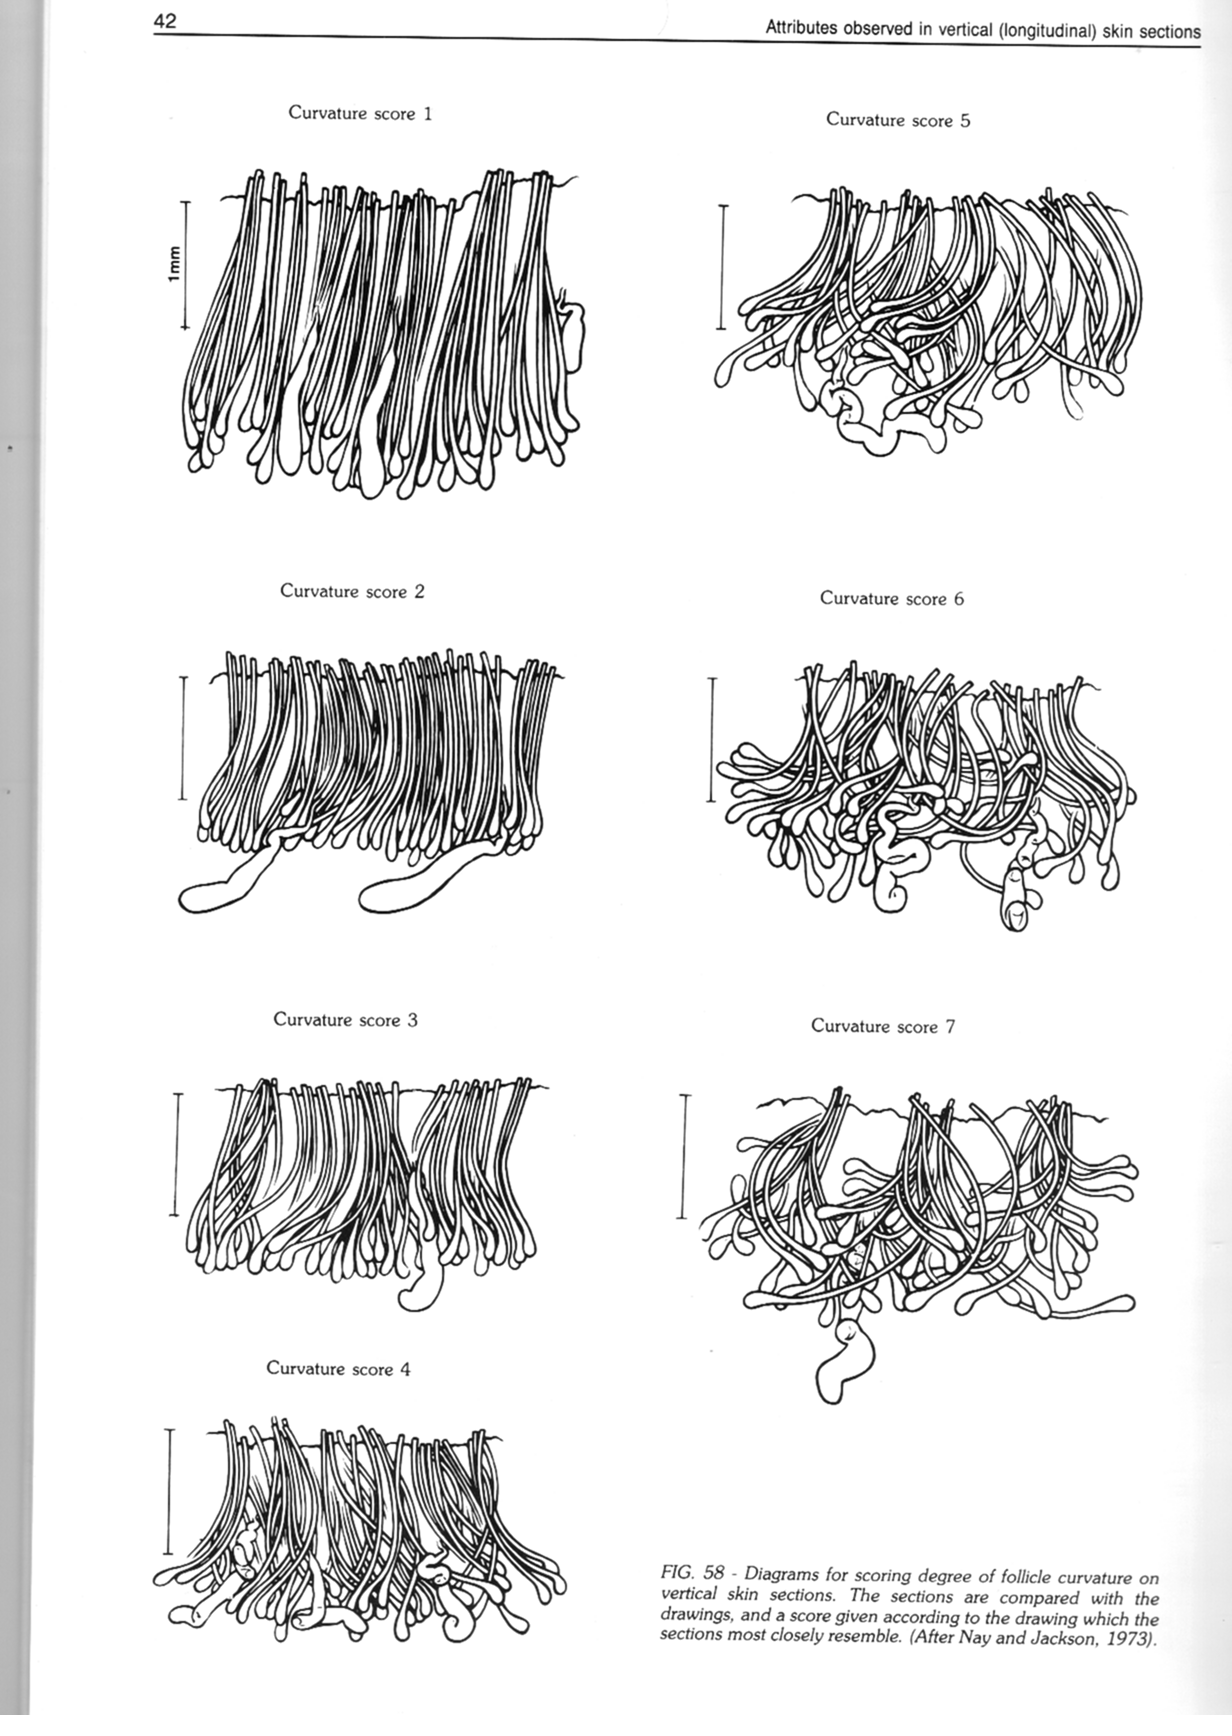
\includegraphics[width=1.0\textwidth]{follcurv.png}
  \caption{The Nay follicle curvature score drawings.  Reproduced from Maddocks and Jackson(1988)~\cite{madd:88}}
  \label{fig:follcurv}
\end{figure}

%\end{document}



The papilla cells ( and therefore the sites in the case of P and So follicles) have to be where the follicle bulbs are. For score 1, the bulbs are all at the same level and directly below the emergence point of the fibre at the epidermal surface. No evidence of movement here. For scores 2 and 3, the bulbs are still all at the same level, but are slightly out of line with the emergence point, so the follicles have a curve, and the sites/papilla cells have moved slightly sideways. For scores 4, 5, 6, and 7 the bulbs are not all at the same level. So do the sites move vertically as well as sideways? It would appear so.  The bulbs are also increasingly out of line with the emergence point, so the follicles curve increasingly, as the scores increase. The sites move sideways as well as vertically. 

What are these follicles in scores 6 and 7 for which the bulb is above the lowest point of the follicle curve and facing upwards?  They would have to be follicles for which the site ( or aggregate of papilla cells) has moved sideways and probably upward after the downgrowth of epidermal tissue has commenced.  They start out straight, then have to curve 'late' in their development, producing the typical 'J' curve with a straight upper shaft and a late curve at the lower end.
 
We have to remember that not all follicles have a site. The Sd follicles  do have a papilla cell aggregate. We do not know  what if anything controls where these Sd aggregates form, but they  seem to cluster alongside existing follicles. We do not know if these Sd papilla cell clusters move, or even if they all form at the same level vertically. So it is difficult to say which might be the Sd follicles in Figure~\ref{fig:follcurv}. There are no distinguishing features - the follicles all look the same. We just know that most of the follicles are Sd's. So what does this suggest. Maybe the Sd follicles are subject to the same papilla cell aggregate movement as the other follicles . Maybe they simply form all over the place initially. 

That is about all we can get out of vertical section from adults. If we had vertical sections of foetal skin we might actually be able to see directly whether follicles curve as they grow. The alternative is that they are bent around afterwards - that still involves movig the 'site', but it also involves dragging the whole fully formed follicle around, which seems biologically unlikely.

We can also have a look at what effects site movement might have on the arrangement of follicles in horizontal sections. We have to bear in mind that horizontal sections are conventionally taken at sebacious gland level, which is well above the bulb region, so any effect of site movement will be minimal. We have to also bear in mind that  follicles and follicle groups are also moved around by expansion of the skin as the animal grows. 

There are some known differences in follicle group arrangement between SRS Merinos and normal wrinkly Merinos.  SRS Merinos tend to have small follicle groups but with a lot of follicles packed into the small group space, that is a high within group density. These small SRS groups tend to be arranged in very ordered rows with wide spaces ( called 'laneways') between the rows containing non-follicle tissue. Whether this more ordered arrangement of follicle groups has  anything to do with absence of site movement is not clear.  What is more likely is that the absence of site movement ( and therefore low follicle curvature) and the ordered groups, and the absence of wrinkle, are all caused by the lack of hard collagen development.  We should consider installing  hard collagen development as a common cause of wrinkle, disordered groups, and site movement with its consequent follicle curvature. This is being dealt with elsewhere (Watts(2018)~\cite{watt:18} in far greater detail.

One observation which comes out in the study referred to above is that hard collagen develops in a layer below the follicle bulbs, but sometimes in extremely wrinkled sheep, it also develops around the follicle bulbs, that is it 'invades' the follicular layer. This would tie in with what we see in the follicle curvature drawings above - the extreme grade 7 score diagram shows follicle bulbs (presumably with their papilla cells) moved around extensively in both the sideways and vertical direction. The hard collagen has to be in amongst those bulbs for it to influence their position, because it has to move the papilla cells to those positions as the follicles are growing.

Well that is about all of the clues to site movement. One of the difficulties is that we are only talking about the sites of P and So follicles being moved. Most of the follicles in Merinos are Sd follicles. We have no idea what affects the placement of the papilla cell aggregates that initiate Sd follicles. We just know that they cluster around other follicles. Because Sd follicles are in greater numbers, what happens to them tends to swamp any effects of P and So follicle placement. 

So can we solve the 'great site movement' mystery? Only partially. We cant finish the detection story with a clear cut answer. It will come out eventually, but not with existing observations. We need a direct measure of 'site movement'. The nearest thing we have to a measure of follicle bulb displacement is the observation of the sagitta (h) of the follicle arc. A large sagitta means the follicle bulb has been displaced, but sagitta is obviously also related to curvature, so it is not a 'clean' measure.  We will just have a brief look at sagitta by plotting curvature ( ie 1/radius of curvature) against curved length of each follicle, with each point shown as the sagitta value. This graph is shown in Figure~\ref{fig:curvxcurvlenxh}.
%\documentclass{article}
%\usepackage{graphicx,subfigure}
%\begin{document}

\begin{figure}[!h]
  \centering
  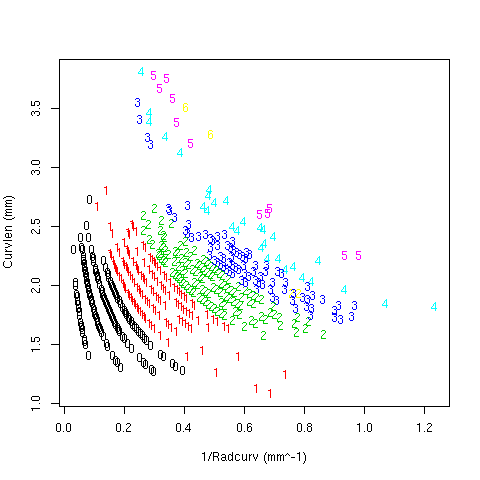
\includegraphics[width=1.0\textwidth]{curvxcurvlenxh.png}
  \caption{Plot of  1/Radius of curvature against curved length of follicles. The sagitta height (h) is shown as point labels which are sagitta height scaled by 10}
  \label{fig:curvxcurvlenxh}
\end{figure}

%\end{document}


 Clearly if sagitta measures bulb displacement, then the most displaced bulbs are both longer follicles and more curved follicles. That is what we have already concluded. So maybe sagitta does measure site movement.  Anactual measure of bulb displacement would be better, but we must not forget that thick vertical sections are 3D objects. All our measurements - straight length (t) and sagitta (h) are 2D projections and therefore biased. All the calculations we make from the measrements - curved length and radius of curvature - are also biased. A bulb displacement measure would also be biased. 

We must not be carried away with the apparent order of Figure~\ref{fig:curvxcurvlenxh}. It represents a family of curves of equal 'h' value. It is like that because bothe Curvlen and Radcurv are calculated from 'h' ( and 't') by our equations. The separation of the lines of equal 'h' value is simply a property of our equations. We chose to use 1/Radcurv in Figure~\ref{fig:curvxcurvlenxh}, rather than Radcurv as in Figure~\ref{fig:radcurvxcurvlen} simply because it displays the sagitta effect better. So where are the P and So follicles in Figure~\ref{fig:curvxcurvlenxh}? They do not cluster separately as in Figure~\ref{fig:radcurvxcurvlen}, but the loose skin P and So follicles are in the bottom left corner ( with a low sagitta value ), and the wrinkly skin P and So follicles are towards the top right corner along the lines with large sagitta value representing lots of bulb displacement. The bulk of follicles in the middle are Sd's, and probably also follicles which curve out of the plane of measurement.

Finally, what Figure~\ref{fig:curvxcurvlenxh} shows is that sagitta is not just curvature, but a range of combinations of curved length and curvature. Moving the site does cause follicles to curve, but it also causes them to grow longer in order to reach the displaced site. So maybe sagitta is a good measurement of site movement. We will have to think about it.


\clearpage
\begin{thebibliography}{99}

\bibitem{bogo:40}
 Bogolyubsky S.N. (1940) cited by Fraser A.S and Short B.F. (1960) The Biology of the Fleece. Animal Research Laboratories Technical Paper No 3. CSIRO Melbourne 1960.


\bibitem{cart:43}
Carter H.B. (1943) Studies in the biology of the skin and fleece of sheep. 1. The development and general histology of the follicle group in the skin of the Merino. 2. The use of tanned sheepskin in the study of follicle population density. 3. Notes on the arrangement, nomenclature, and variation of skin folds and wrinkles in the Merino. C.S.I.R. Bulletin No 164, Melbourne, 1943

\bibitem{fras:60}
Fraser A.S and Short B.F. (1960) The Biology of the Fleece. Animal Research Laboratories Technical Paper No 3. CSIRO Melbourne 1960.


\bibitem{jack:17a}
Jackson, N. (2017) Genetic relationship between skin and wool traits in Merino sheep. Part I Responses to selection and estimates of genetic parameters. URL https://github.com/nevillejackson/Fleece-genetics/tree/master/skinandfleeceparameters/ab3220/skinwool1.pdf

\bibitem{jack:18}
Jackson, N. and Watts, J.E. (2018) Does follicle development affect the spatial layout of sheep skin? URL https://github.com/nevillejackson/Fleece-biology/tree/master/skinspace/skinspace.pdf


\bibitem{jack:17b}
Jackson, N. and Watts, J.E. (2017) What is known about the genetics of wrinkle score in Merino sheep? URL https://github.com/nevillejackson/Fleece-genetics/wrinkle/wrinkle.pdf

\bibitem{knig:93}
Knight, K.R., Lepore, D.A., Horne, R.S., Ritz, M., Kumta, S. and O'Brian, B.M. (1993) Collagen content of uninjured skin and scar tissue in foetal and adult sheep. Int. J. Exp. Pathol. 74(6):583-591

\bibitem{madd:88}
Maddocks, I.G. and Jackson, N. (1988) Structural studies of sheep, cattle, and goat skin. CSIRO, Division of Aimal Production, Sydney.

\bibitem{ment:80}
Menton, D.N. and Hess, R.A. (1980) The ultrastructure of collagen in the dermis of tight-skin (Tsk) mutant mice. The Journal of Investigative Dermatology 74:139-147

\bibitem{mitc:84}
Mitchell, T.W. et al (1984) Some physical and mechanical properties of sheep akin with a comparison of "thick" and "thin" skins. Wool Technology and Sheep Breeding, Vol XXXII, No IV, 200-206


\bibitem{nay:66}
Nay, T. (1966) Wool follicle arrangement and vascular pattern in the Australian Merino. Aust. J. Agric. Res. 17:797-805

\bibitem{rprog:13}
R Core Team (2013). R: A language and environment for statistical
  computing. R Foundation for Statistical Computing, Vienna, Austria.
  ISBN 3-900051-07-0, URL http://www.R-project.org/.


\bibitem{watt:17}
Watts, J.E., Jackson, N., and Ferguson, K.A. (2017) Improvements in fleece weight weight and wool quality of Merino sheep selected visually for high fibre density and length. URL https://github.com/nevillejackson/SRS-Merino/Paper\_2\_Revised\_10\_November\_2017.docx 

\bibitem{watt:18}
Watts, J.E. (2018) Personal communication

\end{thebibliography}
\end{document}
